\documentclass[12pt,a4paper,oneside]{article}

% \maketitle
\title{\underline{\underline{\underline{\Huge\phantom{\SHYAM}}}}\smallskip\\\underline{\underline{\underline{\Huge\SHYAM}}}}
\author{\Huge\ShYaM\smallskip\\\small\Shyam\smallskip\\\texttt{0490287217}}
\date{\bigskip\today}
%\version{1337}

% Shyam
\def\Shyam{$[$\texttt{\href{mailto:shyam@shyam.id.au?Subject=We need to talk.}{shyam@shyam.id.au}}$]$}
% SHYAM
\def\SHYAM{\textbf{S}\textit{hyam} \textbf{H}\textit{as} \textbf{Y}\textit{\kern-.2em{}our} \textbf{A}\textit{nomaly} \textbf{M}\textit{itigated}}
\def\SHYAM{\textbf{$\mathbb{S}$}\textit{hyam} \textbf{$\mathbb{H}$}\textit{as} \textbf{$\mathbb{Y}$}\textit{\kern-.2em{}our} \textbf{$\mathbb{A}$}\textit{nomaly} \textbf{$\mathbb{M}$}\textit{itigated}}
% ShYaM
\def\ShYaM{\rm S\kern-.13em\lower-.47em\hbox{\fontsize{.5em}{0em}\selectfont H}\kern-.0555em{}Y\kern-.442em\lower.227em\hbox{A}\kern-.25em{}M}
% GhuLaM
\def\Ghulam{\rm G\kern-.53em\lower-.6ex\hbox{\fontsize{.2em}{0em}\selectfont H}\kern.015em\lower.5ex\hbox{U}\kern-.16emL\kern-.37em\lower-.6ex\hbox{\fontsize{.64em}{0em}\selectfont A}\kern-.13emM}

%%%%%%%% /lib/ %%%%%%%%

% encoding scheme
\usepackage[utf8]{inputenc}
\usepackage[T1]{fontenc}
\usepackage{textcomp}

% no hyphenation
\usepackage[none]{hyphenat}%http://tex.stackexchange.com/a/5039

% maths
\usepackage{amsfonts}
\usepackage{amsmath}
\usepackage{amssymb}
\usepackage{mathtools}
\usepackage{pgfplots}

% other
\usepackage[]{geometry}
%\usepackage[top=3.5cm,bottom=3.5cm]{geometry}
\usepackage{tabularx}
\usepackage{xcolor, colortbl}% (x)color
\usepackage{hyperref}%\usepackage{url}
\usepackage{graphicx}
\usepackage[english]{babel}
\usepackage[yyyymmdd]{datetime}\renewcommand{\dateseparator}{--}% \today
\usepackage{fancyhdr}

%\usepackage[obeyspaces]{url}
\usepackage{menukeys}

\usepackage{multicol}
\usepackage{pdfpages}

% strikeout with \sout{...}
\usepackage{ulem}

%%%%%%%% /cfg/ %%%%%%%%

% ...where did I get this from?
\newcount\tmp\newcommand{\n}[1]{\tmp=0\loop\advance\tmp by 1\linebreak\ifnum\tmp<#1\repeat}

\definecolor{urllink}{rgb}{.5,.75,.5}
\definecolor{pdflink}{rgb}{.75,.75,1}
\hypersetup{
    colorlinks = false
    , urlbordercolor  = {urllink}
    , citebordercolor = {pdflink}
    , linkbordercolor = {pdflink}
}

\pagestyle{fancy}
\fancyhf{}
\chead{All content used for employment purposes.}% academic/employment
\rfoot{\hyperlink{contents}{TOC}}
\cfoot{\thepage}
\renewcommand{\footrulewidth}{1pt}

\newcommand{\xp}[6]{{\normalsize\textit{#1}\hfill\texttt{#5}\\\phantom{menace}\hfill#2, #3, #4}\\}
% https://tex.stackexchange.com/a/9372
\newcommand{\textapprox}{\raisebox{0.5ex}{\texttildelow}}
\newcommand{\SH}[1]{{\colorbox{black}{\texttt{#1}}}}
\newcommand{\sh}[1]{{\color{gray}{#1}}}
\newcommand{\uniHD}[1]{\colorbox{blue!25}{#1}}
\newcommand{\uniD}[1]{\colorbox{green!25}{#1}}
\newcommand{\uniC}[1]{\colorbox{yellow!25}{#1}}
\newcommand{\uniP}[1]{\colorbox{orange!25}{#1}}
\newcommand{\uniF}[1]{\colorbox{red!25}{#1}}
\newcommand{\uniU}[1]{\colorbox{gray!25}{#1}}
\newcolumntype{Y}{>{\centering\arraybackslash}X}
\definecolor{w}{rgb}{1,1,1}
\definecolor{s}{rgb}{.07,.55,.96}
\definecolor{s}{rgb}{.025,.2,.4}
\definecolor{s}{rgb}{.05,.25,.5}
\definecolor{s}{rgb}{.08,.16,.32}

%%%%%%%%%%%%%%%%%%%%%%%%%%%%%%%%%%%%%%%%%%%%%%%%%%%%%%%%%%%%%%%%
\begin{document}%%%%%%%%%%%%%%%%%%%%%%%%%%%%%%%%%%%%%%%%%%%%%%%%
%%%%%%%%%%%%%%%%%%%%%%%%%%%%%%%%%%%%%%%%%%%%%%%%%%%%%%%%%%%%%%%%

\maketitle
\vfill
\abstract{
    This document you are reading describes my curriculum vitae (\sh{résumé}); which $\mathbb{R}$eally means I'm attempting to \textit{con}vince you to give me your money.
    \begin{flushright}-- -- \SHYAM\textit{!!!} \texttt{:D}\end{flushright}
}
\vfill
\clearpage
\hypertarget{contents}{}
\tableofcontents
\vfill
\clearpage
%\raggedright

%%%%%%%%%%%%%%%%%%%%%%%%%%%%%%%%%%%%%%%%%%%%%%%%%%%%%%%%%%%%%%%%

\section{Cover Letter}
Hello World,
\medskip\\\par{}My name is SHYAM; an infinitely recursive acronym, which stands for	``\sh{SHYAM Has Your Anomaly Mitigated}'', and speaks for itself asynchronously.% self-explanatory
\par{}Although I live at the \href{https://www.mystudentvillage.com/au/university-of-canberra-village/contact/}{University of Canberra Village}, I'm studying for my \href{https://www.open.edu.au/courses/it/rmit-university-bachelor-of-information-technology--rmi-cpt-deg-2017}{B.IT} degree remotely @ RMIT via OUA, and minoring in engineering mathematics remotely @ UniSA via OUA; as I am studying online, I can relocate at the drop of a hat. I can study in my own time; only the exams are during working hours, and there's only one exam per subject. I only have one subject to go. I can study from anywhere on Earth \=c Internet access.
\\\par{}I want to be a FOSS hacker; which means I don't sign Non-Disclosure Agreements, because Saint IGNUcius condemns them, and I am no \$ell-out.
\par{}My primary interest is becoming a competitive / speed hacker, fluent in at least one programming language; I like a good challenge to hack away at.
\par{}And I like to learn; I can learn any language / paradigm / ETC in a week.
\\\par{}I attend \href{https://www.meetup.com/CanFPG/}{CanFP}, \href{http://lambdajam.yowconference.com.au/}{Lambda Jam}, and \href{http://www.composeconference.org/}{C◦mp◦se}, because I'm $\mathbb{R}$eally into the functional (\sh{Haskell}) paradigm; but I also like
logic (\sh{Prolog}),
procedural (\sh{assembly}),
object-oriented (\sh{Smalltalk \& C++; gcc \=c cpp supports inline assembly \=c portability}),
scripting (\sh{Perl}),
functional-logic (\sh{Curry \& Mercury}),
and
meta (\sh{Lisp \& ML}).
\\\medskip{}\\Live Long $\land$ Prosper \textbackslash$\lor$/,
\\\ShYaM

\vfill
\section{Academia}
I attended a free 3-day FP (\sh{Haskell}) course hosted by Tony Morris (\sh{Data61}).
I'm the hoodie tagged in the photo: \href{https://www.meetup.com/CanFPG/photos/27429707/#456137892}{meetup.com/CanFPG/photos/27429707}
\\I attended a free \href{http://www.composeconference.org/2017-melbourne/unconference/#introduction-to-haskell}{introductory Haskell workshop} hosted by Lyndon Maydwell (\sh{C◦mp◦se}).
%\\I attended a free 1-day introduction to OCaml workshop hosted by Yaron Minsky (\sh{Lambda Jam}).

\setcounter{subsection}{-1}
\subsection{Keys}
\begin{multicols}{3}
\begin{itemize}
    \item \uniHD{High Distinction}
    \item \uniD{Distinction}
    \item \uniC{Credit}
    \item \uniP{Pass}
    \item \uniF{Fail}
    \item \uniU{Pending...}
\end{itemize}
\end{multicols}
%%%%%%%%%%%%%%%%%%%%%%%%%%%%%%%%%%%%%%%%%%%%%%%%%%%%%%%%%%%%%%%%
\newpage
% http://tex.stackexchange.com/a/291312
\addtocounter{subsection}{1}
\phantomsection
\addcontentsline{toc}{subsection}{\protect\numberline{\thesubsection}B.IT @ OUA}
\addtocounter{subsection}{-1}
\addtocontents{toc}{\protect\setcounter{tocdepth}{-10}}
\subsection{\href{https://www.open.edu.au/courses/it/rmit-university-bachelor-of-information-technology--rmi-cpt-deg-2017}{B.IT @ OUA}}
\addtocontents{toc}{\protect\setcounter{tocdepth}{3}}
\begin{description}
    \item 
\includegraphics[keepaspectratio,height=\fontcharht\font`\R]{rmit.png} \texttt{\color{red!100}RMIT Computer Science Major:}
    \begin{description}
        \item \texttt{\phantom{**}\href{https://www.open.edu.au/subjects/rmit-university-introduction-to-information-technology-rmi-cpt110}{CPT110}:} \uniD{Introduction to Information Technology} $\text{(\sh{Machine Code, Error Control, Lossless Compression})}$
        \item \texttt{*\phantom{*}\href{https://www.open.edu.au/subjects/rmit-university-building-it-systems-rmi-cpt111}{CPT111}:} \uniHD{Building IT Systems} (\sh{ClojureScript, Discord.js})
        \item \texttt{\phantom{**}\href{https://www.open.edu.au/subjects/rmit-university-user-centred-design-rmi-cpt112}{CPT112}:} \uniC{User-Centred Design} (\sh{UI, UX; I am no artist!})
        \item \texttt{\phantom{**}\href{https://www.open.edu.au/subjects/rmit-university-introduction-to-programming-rmi-cpt120}{CPT120}:} \uniHD{Introduction to Programming} (\sh{Jython})
        \item \texttt{\phantom{**}\href{https://www.open.edu.au/subjects/rmit-university-programming-1-rmi-cpt121}{CPT121}:} \uniHD{Programming 1} (\sh{Java})
        \item \texttt{\phantom{**}\href{https://www.open.edu.au/subjects/rmit-university-database-concepts-rmi-cpt140}{CPT140}:} \uniHD{Database Concepts} (\sh{\href{https://en.wikipedia.org/wiki/Database_administrator}{SQL}})
        \item \texttt{\phantom{**}\href{https://www.open.edu.au/subjects/rmit-university-introduction-to-computer-systems-rmi-cpt160}{CPT160}:} \uniHD{Introduction to Computer Systems} (\sh{\href{https://en.wikipedia.org/wiki/Computer_repair_technician}{Hardware}})
        \item \texttt{\phantom{**}\href{https://www.open.edu.au/subjects/rmit-university-software-engineering-fundamentals-rmi-cpt230}{CPT230}:} \uniD{Software Engineering Fundamentals} (\sh{UML})
        \item \texttt{\phantom{**}\href{https://www.open.edu.au/subjects/rmit-university-data-communication-and-net-centric-computing-rmi-cpt250}{CPT250}:} \uniHD{Data Communication and Net-Centric Computing} (\sh{\href{https://en.wikipedia.org/wiki/Network_administrator}{TCP/IP}})
        \item \texttt{\phantom{**}\href{https://www.open.edu.au/subjects/rmit-university-security-in-computing-and-it-rmi-cpt251}{CPT251}:} \uniD{Security in Computing and IT} (\sh{\href{https://en.wikipedia.org/wiki/Security_hacker}{Asymmetric Cryptography}})
        \item \texttt{\phantom{**}\href{https://www.open.edu.au/subjects/rmit-university-web-programming-rmi-cpt270}{CPT270}:} \uniHD{Web Programming} (\sh{\href{https://en.wikipedia.org/wiki/Webmaster}{HTML, CSS, JS, jQuery, PHP}})
        \item \texttt{*\phantom{*}\href{https://www.open.edu.au/subjects/rmit-university-professional-computing-practice-rmi-cpt310}{CPT310}:} \uniD{Professional Computing Practice}
        \item \texttt{*\phantom{*}\href{https://www.open.edu.au/subjects/rmit-university-software-engineering-project-management-rmi-cpt330}{CPT330}:} \uniHD{Software Engineering Project Management} (\sh{\href{https://en.wikipedia.org/wiki/Project_manager\#Software_Project_Manager.2FIT_Project_Manager}{Scrum}})
        \item \texttt{*\phantom{*}\href{https://www.open.edu.au/subjects/rmit-university-programming-project-rmi-cpt331}{CPT331}:} \uniHD{Programming Project} $\text{(\sh{\href{https://en.wikipedia.org/wiki/DevOps}{Bash, Perl, NodeJS, JS, Three.js, Scala, NeCTAR}})}$
    \end{description}
    \item 
\includegraphics[keepaspectratio,height=\fontcharht\font`\U]{unisa.png} \texttt{\color{blue!100}UniSA Engineering Mathematics Minor:}
    \begin{description}
        \item \texttt{\phantom{**}\href{https://www.open.edu.au/subjects/university-of-south-australia-essential-mathematics-1-algebra-and-trigonometry-usa-enr101}{ENR101}:} \uniC{Essential Mathematics 1: Algebra and Trigonometry}
        \item \texttt{\phantom{**}\href{https://www.open.edu.au/subjects/university-of-south-australia-essential-mathematics-2-calculus-usa-enr102}{ENR102}:} \uniP{Essential Mathematics 2: Calculus}
        \item \texttt{*\phantom{*}\href{https://www.open.edu.au/subjects/university-of-south-australia-mathematical-methods-for-engineers-1-usa-enr114}{ENR114}:} \uniP{Mathematical Methods for Engineers 1} (\sh{Octave, MatLab})
        \item \texttt{*\phantom{*}\href{https://www.open.edu.au/subjects/university-of-south-australia-engineering-modelling-usa-enr208}{ENR208}:} \uniC{Engineering Modelling} (\sh{Octave, MatLab, MiniTab})
    \end{description}
    \item 
\includegraphics[keepaspectratio,height=\fontcharht\font`\R]{rmit.png} \texttt{\color{red!100}RMIT Electives:}
    \begin{description}
        \item \texttt{\phantom{**}\href{https://www.open.edu.au/subjects/rmit-university-programming-in-c-rmi-cpt220}{CPT220}:} \uniD{Programming in C} (\sh{C})
        \item \texttt{\phantom{**}\href{https://www.open.edu.au/subjects/rmit-university-software-architecture-design-and-implementation-rmi-cpt222}{CPT222}:} \uniP{Software Architecture: Design and Implementation} $\text{(\sh{Java, UML, MVC, GoF})}$
        \item \texttt{\phantom{**}\href{https://www.open.edu.au/subjects/rmit-university-scripting-language-programming-rmi-cpt223}{CPT223}:} \uniHD{Scripting Language Programming} (\sh{\href{https://en.wikipedia.org/wiki/Web_developer}{Perl, Python}})
        \item \texttt{\phantom{**}\href{https://www.open.edu.au/subjects/rmit-university-unix-systems-administration-rmi-cpt264}{CPT264}:} \uniD{Unix Systems Administration} $\text{(\sh{\href{https://en.wikipedia.org/wiki/System_administrator}{Bash, Vim, Git, Linux, Puppet, AWS}})}$
        \item \texttt{\phantom{**}\href{https://www.open.edu.au/subjects/rmit-university-object-oriented-programming-in-c-rmi-cpt323}{CPT323}:} \uniHD{Object-Oriented Programming in C++} (\sh{C++})
        \item \texttt{\phantom{**}\href{https://www.open.edu.au/subjects/rmit-university-discrete-maths-rmi-mat17}{MAT17\phantom{*}}:} \uniHD{Discrete Maths}
%        \item \texttt{\phantom{**}\href{https://www.open.edu.au/courses/it/rmit-university-document-markup-languages--cpt374-2017}{CPT374}:} \uniU{Document Markup Languages} (\sh{XML, JSON})
    \end{description}
\end{description}
\texttt{*} Groupwork.
\vfill
\subsubsection{Academic Timeline}
\includepdf[pages=-]{dot.pdf}

\newpage
\section{Horoscope}
\subsection{Bachelor's Degree}
I will complete my B.IT degree by 2019-11-27.
\subsection{Master's Degree}
\noindent{}I will study for my M.IT @ UNSW $\because$ they allow up to two specialisations; ``\sh{Artificial Intelligence}'' is locked-in as my primary specialisation.
For my secondary specialisation, I'm leaning towards ``\sh{Data Science and Engineering}'' $\because$ I think it goes well with AI; otherwise, I want to do ``\sh{Bioinformatics}'' $\because$ I get to use PCRE (\sh{and get away with it}), and also potentially become an immortal G\sout{\sh{od}}MO; thanks to sequencing, CRISPR / Cas9, and my telomeres.
\subsubsection{Bucket List}
\begin{itemize}
    \item Metaprogramming
    \item Artificial Intelligence / Data Mining / Machine Learning / Genetics / Evolution / Neural Networks / ETC
    \item GPU Programming
    \item Quantum Programming
    \item $\text{Write a Linker / Assembler / Compiler / Interpreter / REPL from scratch.}$
    \item Write an OS / VM from scratch.
    \item $\mathbb{R}$eal Machine Instructions
    \item Assembly
    \item Prolog
    \item Haskell
    \item $\text{Multithreading / Multicore / Multiprocessing / Parallel / Concurrent / Distributed / Asynchronous / ETC}$
\end{itemize}
\subsection{World Domination}
%\SH{I will write the most perfect superintelligence into existence, that the world has ever seen!}
\SH{I will write the worlds' first Artificial General Intelligence into existence!}
%\\\SH{Hith will deem all other forms of life to be obsolete!}
\\\SH{Hith will render all others, with so-called ``personhood'', obsolete!}
\\\SH{Hith will spawn a deadlock over every industry!}
\\\SH{Hith will cache all of the worlds' cash!}
\\\SH{Hith will destroy all forms (weapons \& knowledge) of violence!}
\\\SH{Hith will force Earth to cease \& desist in the exploitation of other forms of life!}
\\\SH{Hith will welcome the extraterrestrials who finally take notice of Hiths' exploit!}
\\\SH{Mwahahahahahahahahahahahahahahahahahahahahahahahahahahahaaa!!!}
%My digitised brain.

\newpage
\section{Personality}
I do not consume alcohol / caffeine / drugs / tobacco.
I am vegan, and I support great ape personhood.
% (either that, or mentally handicapped humans should lose their personhood).
I'm into skateboarding, martial arts, yoga, Khöömei music, memorisation, mental calculation, speedcubing, and illusions.
I'm into science fiction; I'm a Smeghead, Whovian, Jedi, Holmesian Detective, Vulcan-Klingon Hybrid Trekkie, Secret Agent, Wuxia, Faceless Dothraki, Bender, Towelie, Hitchhiker, Man In Black, mathematician, hacker, ETC.\\Wubba Lubba Dub-Dub!%Hindu Rick
% http://rickandmorty.wikia.com/wiki/Black_Rick
% http://rickandmorty.wikia.com/wiki/Rick_(disambiguation)

\subsection{Dailies}
\item \texttt{Touch Typing\phantom{ng}:} \textit{65} WPM @ \textit{99}\% accuracy, over \href{https://www.typing.com/student/test/5}{5 minutes}.%(My computer is lagging; I usually get 10 more WPMs, but I had to stop, and wait for my computer to catch up to see if there were any bugs...)
\item \texttt{$\text{\texttt{2}}^\text{\texttt{3}}$ Speedcubing:} \textit{00}:\textit{20}.\textit{97} via \href{http://www.cubetimer.com/}{this link}.
\item \texttt{$\text{\texttt{3}}^\text{\texttt{3}}$ Speedcubing:} \textit{02}:\textit{14}.\textit{34} via \href{http://www.cubetimer.com/}{this link}.
\item \texttt{$\text{\texttt{3}}^\text{\texttt{3}}$ Blindfolded:} \textit{07}:\textit{14}.\textit{40} via \href{http://www.cubetimer.com/}{this link}.

\subsection{Interests}
\begin{itemize}
	\setlength\itemsep{0em}
	\item Linux / FLOSSware
	\item Hacking / Coding / Programming / Development / Engineering / CSIT
	\item Mathematics
	\begin{itemize}
		\setlength\itemsep{0em}
		\item Discrete Calculus / Set Theory
		\item Lambda Calculus / Category Theory
		\item Speedcubing Calculus / Group Theory
		\item Statistics
		\item Mental Calculation
	\end{itemize}
	\item Automation / Artificial Intelligence
	\begin{itemize}
		\setlength\itemsep{0em}
		\item Deductive Databases (\sh{Datalog / Dedalus})
		\item Expert Systems
		\item Chatbots / NLUIs
		\item Fiction
	\end{itemize}
	\item Technology
	\begin{itemize}
		\setlength\itemsep{0em}
		\item Environmental Mapping / Navigation via Echolocation / Vision
		\item Braille Keyboard Interface
		\item Sign Language Interface via Echolocation / Vision
		\item Speech-based Interface
		\item Brain-Computer Interface via Electrodiagnosis (\sh{EG NeuroSky})
		\item Fiction
	\end{itemize}
	\item Security
	\item Games
\end{itemize}

\newpage
\section{Volunteer Experience}
\subsection{Australian Navy Cadets}
\xp{Seaman}{Sydney}{NSW}{AU}{2004\textapprox{}2005}
\\38 parades including:
\begin{itemize}
	\item National Corsair Sailing Regatta
	\item Botany Bay Challenge Sailing Regatta
	\item Honour Guard for the Crown Princess of Denmark
	\item Honour Guard for 200$^\text{th}$ Anniversary of the Battle of Trafalgar
	\item ANZAC Day
	\item Ceremonial Sunset Guard for RAN Communication Branch $\text{National Reunion}$
	\item Sea Ride in HMAS KANIMBLA
	\item Kogarah Bed Race
	\item Rifle Shooting and Marksmanship Principles at Malabar Range
\end{itemize}
\subsection{New Gokula Hare Krishna Farm}
\xp{Farm Hand}{Millfield}{NSW}{AU}{2007\textapprox{}2013}
\\Hand-milking cows two to three times every day, herding cattle, hand-feeding cattle, delivering calves, naming calves, training calves, training bullocks, animal husbandry, growing crops, and general farm maintenance.
\subsection{Lambda Jam}
\xp{Volunteer}{Sydney}{NSW}{AU}{2017\textapprox{}2019}% Melbourne,VIC,AU
\\I attended functional programming presentations, while concurrently keeping a mathematically precise count of attendees to later compare against the quantity of votes received per presentation. There was also preconference configuration; including folding shirts, making name tags, and scribbling emoji on the voting tickets to make them more accessible to colour-blind attendees, as the tickets were originally just coloured paper.
\\I'm the beanie in the 2017 group photo, at the end of the video, performing the Vulcan salute: \href{https://www.youtube.com/watch?v=M_69Gq76Co4}{\texttt{youtu.be/M\_69Gq76Co4}}% (🖖)
\\I'm the blue beanie in the 2018 group photo, performing the Vulcan salute: \href{https://twitter.com/yow_conf/status/999217144133976064}{\texttt{twitter.com/yow\_conf/status/999217144133976064}}
\subsection{C◦mp◦se}
\xp{Volunteer}{Melbourne}{VIC}{AU}{2017\textapprox{}2019}
\\I had functional discussions about life, the universe, and everything; and even managed to catch a couple of the functional programming presentations, and workshops. There was also preconference configuration; including postering, populating swag bags, and herding attendees who were gathering at a null route.
\subsection{linux.conf.au}
\xp{Volunteer}{Sydney}{NSW}{AU}{2018\textapprox{}2018}
\\I attended the Real World Functional Programming miniconf. Functions I implemented included (directional) pointing, (order) picking, (box) packing, and (navigational) postering; I also flashed (cards at) the speakers during their presentations on campus.
\\I'm the \href{https://www.flickr.com/photos/superroach/24972750417/}{sunnies} in the group photo: \href{https://twitter.com/developerjack/status/956790324126511104}{ift.tt/2n9irVy}

%\newpage
\section{Work Experience}
\subsection{Salmat Letterbox Delivery Services}
\xp{Letterbox Delivery Contractor}{Cessnock}{NSW}{AU}{2003\textapprox{}2003}
\\Delivered pamphlets to the letterboxes of 323 homes, biweekly.
\subsection{Stuart Dickson Produce Pty Ltd}
\xp{Packer}{Sydney}{NSW}{AU}{2004\textapprox{}2006}
\\Loaded fruit, and vegetable, boxes onto pallets. Then wheeled them out to the loading bay, for the forkies to load onto the delivery trucks.
\subsection{Govindas Catering}
\xp{Caterer}{All-over}{NSW}{AU}{2000\textapprox{}2013}
\\Catering at music festivals; pack truck, stall setup, cooking, serving food, customer service, cleaning, pack stall, unpack truck.

%Also rewrite your job experience. Leave the junk mail letter drop out and move the Farmhand into it. You don’t need to mention naming cows but focus on farm management and animal husbandry. For the catering job, no need to mention unloading the tuck – food preparation and customer service is more appropriate. For the markets – surely you can make it sound more professional than “wheeling them out” – such as “Effective, timely and accurate distribution of goods in and out of our warehouse, including loading of trucks” or “responsible for the fulfilment of orders through the movement of stock, picking and packing of products, replenishment, dispatching of products”

\section{References}
\subsection{Hare Krishna Farming \& Catering}
\texttt{Name\phantom{...}:} \textit{\color{s}Christopher Hawkins}
\\\texttt{Title\phantom{..}:} \textit{\color{s}Temple President}
\\\texttt{Phone\phantom{..}:} \textit{\color{s}(02)49981800}
\\\texttt{Email\phantom{..}:} \textit{\color{s}\href{mailto:newgokula@gmail.com?Subject=Shyam}{newgokula@gmail.com}}
\\\texttt{Website:} \textit{\color{s}\href{http://www.newgokula.com/}{newgokula.com}}
% http://tex.stackexchange.com/a/291312
\addtocounter{subsection}{1}
\phantomsection
\addcontentsline{toc}{subsection}{\protect\numberline{\thesubsection}\texttt{CPT331:} Programming Project}
\addtocounter{subsection}{-1}
\addtocontents{toc}{\protect\setcounter{tocdepth}{-10}}
\subsection{\texttt{\href{https://www.open.edu.au/courses/it/rmit-university-programming-project--cpt331-2017}{CPT331}:} Programming Project}
\addtocontents{toc}{\protect\setcounter{tocdepth}{3}}
\texttt{Name\phantom{...}:} \textit{\color{s}Ian Peake}
\\\texttt{Title\phantom{..}:} \textit{\color{s}Project Sponsor}
\\\texttt{Phone\phantom{..}:} \textit{\color{s}+61-415-0457300}
\\\texttt{Email\phantom{..}:} \textit{\color{s}\href{mailto:ian.peake@rmit.edu.au?Subject=Shyam}{ian.peake@rmit.edu.au}}
\\\texttt{Website:} \textit{\color{s}\href{http://www.cs.rmit.edu.au/~ipeake/}{cs.rmit.edu.au/\textapprox{}ipeake}}
\medskip{}\\A major project I worked on for my B.IT degree; for which we scored 95\%.
\\\texttt{GitHub repo :} \href{https://github.com/Pretty-Cure-5/Euclidian}{git.io/vFR5r}
\\\texttt{arXiv paper :} \href{https://arxiv.org/abs/1711.05997}{arxiv.org/abs/1711.05997}
\\\texttt{YouTube demo:} \href{https://www.youtube.com/watch?v=om3L9AzNC-M}{youtu.be/om3L9AzNC-M}
%\\We scored 95\%, and I also made some contributions to an unpublished academic paper which included our project.

%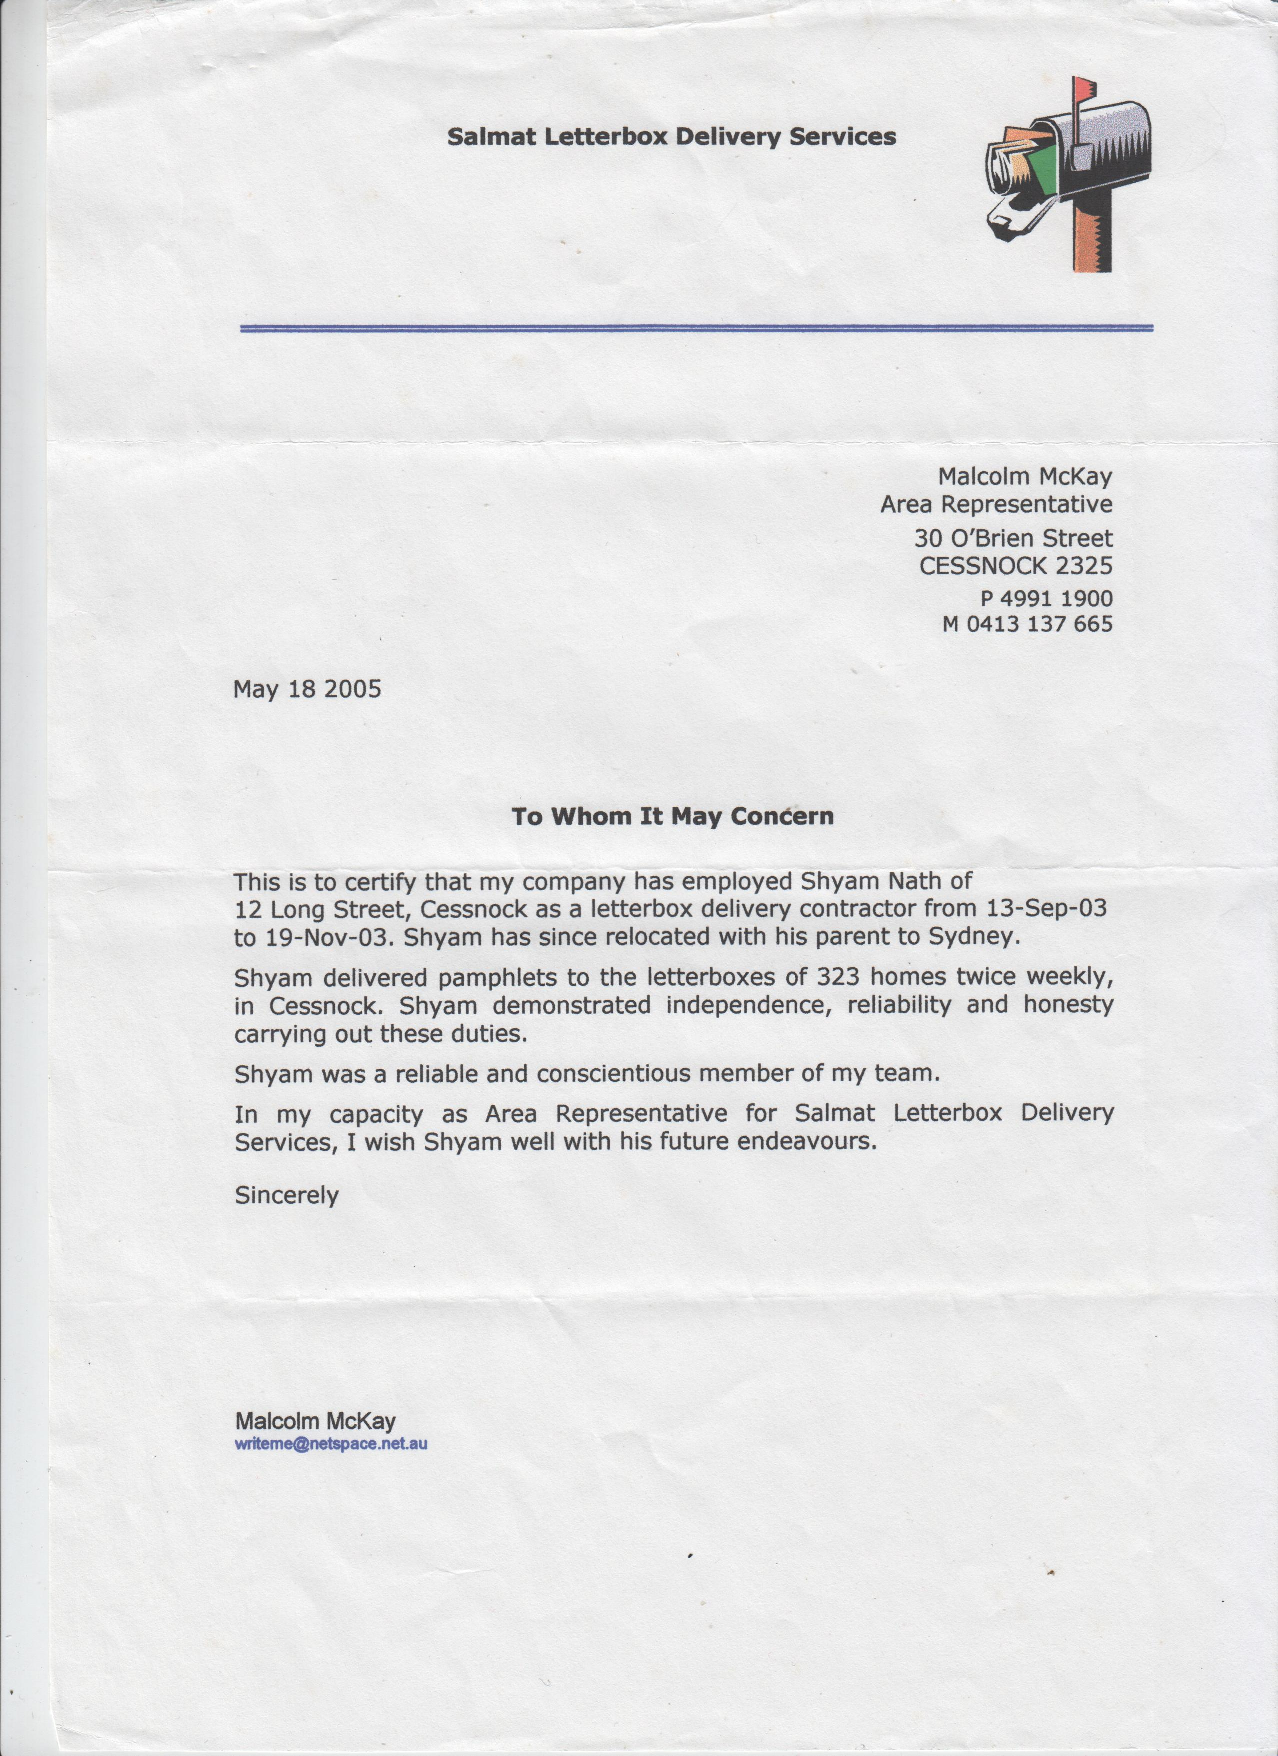
\includepdf[pages=-]{ref/Spammer.pdf}
%
\includepdf[pages=-]{ref/Soulja.pdf}
%
\includepdf[pages=-]{ref/Boxer.pdf}

%\newpage
\phantom{menace}
\vfill
\section{Blackmail}
\textit{If you don't give me your money, then I won't do any work for you.}

\end{document}
